%%
% 引言或背景
% 引言是论文正文的开端,应包括毕业论文选题的背景、目的和意义;对国内外研究现状和相关领域中已有的研究成果的简要评述;介绍本项研究工作研究设想、研究方法或实验设计、理论依据或实验基础;涉及范围和预期结果等。要求言简意赅,注意不要与摘要雷同或成为摘要的注解。
% modifier: 黄俊杰(huangjj27, 349373001dc@gmail.com)
% update date: 2017-04-15
%%

\chapter{绪论}
% 定义,过去的研究和现在的研究,意义
\label{cha:introduction}
\section{选题背景与意义}
\label{sec:background}
% What is the problem
% why is it interesting and important
% Why is it hards, why do naive approaches fails
% why hasn't it been solved before
% what are the key components of my approach and results, also include any specific limitations,do not repeat the abstract
%contribution
% 引言是论文正文的开端,应包括毕业论文选题的背景、目的和意义;对国内外研究现状和相关领域中已有的研究成果的简要评述;介绍本项研究工作研究设想、研究方法或实验设计、理论依据或实验基础;涉及范围和预期结果等。要求言简意赅,注意不要与摘要雷同或成为摘要的注解。

分布式计算框架是一种复杂的平台软件。传统的并行计算范式如信息传递接口(MPI)和分区全局地址空间(PGAS),通常为编程者提供丰富的调用接口和灵活的编程空间。
然而,使用这些编程标准的门槛过高:编程者通常需要自己管理多台机器的状态,特别是内存的分配和使用;编程者还需要使用给定的标准原语,精确地规定多个进程之间的通信和协作方式,
这通常需要大量时间和精力;另外使用这些范式将导致程序和功能的强耦合——编程者很可能不得不重新编写代码来更新程序的逻辑。因此,现代分布式计算框架通常承担了上述硬件管理的角色,
并针对目标任务类型,为用户设计尽可能少、但简单易用的功能接口,来降低集群的使用难度。传统的分布式计算框架,例如Mapreduce和Spark,都是面向大规模数据分析而设计的。然而,近些年
以强化学习、复杂工作流等为代表的复杂计算需求,需要更灵活的框架支持。加州大学伯克利分校RISELab实验室提出的Ray和芝加哥大学Globus实验室提出的Parsl是其中两个典型。这些框架
吸取了云计算领域“函数即服务(Function as a Service, FaaS)”的设计思想,能够细粒度地以函数为单位将任务调度到集群上执行,同时依然对用户隐藏绝大部分实现细节。Ray通过分布式内存对象存储Plasma,
实现了框架完全自主的集群内存管理,让用户可以专注于实现功能逻辑,无需担心数据的存放和移动。Ray在保持易用性的前提下,极大地提升了计算框架的灵活性,用户只需要修改几行代码就能将单进程程序扩展到整个集群,
进而实现分布式机器学习等复杂模型。

高性能集群(或超算集群),是一种以高端处理器、并行加速卡、高性能网络、大容量存储为核心硬件的计算集群。随着大数据应用的丰富、超大规模人工智能模型的出现,高性能集群和超级计算机正在变得愈发重要。
首先,高性能计算机拥有普通机器不能比拟的计算能力,主要表现为高端的多核处理器和并行加速卡。而随着大模型时代的到来,新应用对集群网络的需求快速提高,高性能网络所表现出的高带宽、低延迟等特性
也逐渐受到了更多的关注。当前,高性能计算集群普遍使用的是英伟达Mellanox子公司的Infiniband高速网络。这一网络架构的性能优势,很大程度上来自于对远程直接内存访问(RDMA)机制的支持。
而对于传统使用套接字(Socket)通信的网络程序,该架构通过“基于Infiniband的互联网协议(IPoIB)”实现支持。值得注意的是,这是一种依赖操作系统内核的非原生支持:已经有多个工作表明,
其网络性能和直接使用RDMA技术相比具有明显差距。然而,要利用RDMA,用户必须在应用中实现基于RDMA的通信机制,而不能依赖于操作系统内核提供的系统调用。
因此,基于Socket的网络应用大多不能在高性能集群中直接获得显著的性能提升。分布式计算框架Ray并不例外,其分布式内存存储Plasma目前仅有对传统TCP/IP协议的支持,因而在超算集群上无法发挥出应有的网络性能,
进而影响Ray运行在超算上的总体性能。

因此,本研究的目的是:我们是否能为分布式内存存储Plasma,提出并实现一种支持RDMA机制的内存通信协议,从而让Plasma乃至整个Ray框架在
现代超算集群上获得更好的性能?从超算研究的趋势来说,应用软件和先进超算硬件之间的隔阂,正在逐渐成为大家关注的热点。随着超级计算机和云计算两个领域的融合,会有越来越多的软件运行在高性能集群中。
然而,它们中的大部分还没有针对高性能硬件提供软件支持——通过提供软件对高性能硬件的支持,我们能够将这些应用的运行性能提升到全新的水平。

\section{国内外研究现状和相关工作}
\label{sec:related_work}

\subsection{分布式计算框架}

分布式计算框架是一种复杂的平台软件。在底层,它通过实现任务调度、并发执行、内存管理等基本组件,向用户透明地提供分布式计算的功能;在应用层,它通过设计和规范一系列接口,帮助用户高效地运行特定任务:例如大数据分析(Mapreduce、Spark),
分布式机器学习(Ray)等等。Ray是近年来最受关注的分布式计算框架,它以函数为单位调度任务执行,完全自主地管理内存移动,并且支持异步执行。借助这一平台,目前社区人员已经实现了机器学习(Ray ML)、强化学习(Ray RLlib)、模型部署(Ray Serve)、工作流(Ray Workflows)
等上层应用库供用户使用。同时,用户也可以直接在框架上编写任意程序:使用常见的Python语法构建出完全分布式的计算程序,而且不会有任何表达能力上的限制。

\begin{lstlisting}[style=sysupython, caption=Ray代码示例]
	import ray
	ray.init()
	
	@ray.remote
	def f(x):
	    return x * x
	
	futures = [f.remote(i) for i in range(4)]
	print(ray.get(futures)) # [0, 1, 4, 9]
\end{lstlisting}

在上述代码片段中,用户通过修饰符"@ray.remote"将函数定义为远程函数,并在下方执行4次。值得注意的是,在Ray框架的调度下,这四次调用将会逐一调度到不同的进程上并发执行,因此Ray能够透明地
为任何函数提供并行计算能力。而分布式内存存储Plasma,则在系统中持续为并发任务调度所需的数据。在示例代码中,Plasma将会在集群中查找变量i的位置,并将其拉取到进程中供任务使用。最后,Ray原生支持异步执行,
任何函数调用都会立刻返回,给予用户一个凭证(future)——用户可以立刻用这一凭证作为参数继续调用其他函数,即使数据的真实值还没有求得。Ray的执行引擎动态地构建和解决数据依赖,将凭证替换为真实值,然后继续调用依赖它的函数。
这一异步特性将使Ray充分发挥并发任务的性能。

\subsection{远程直接内存访问技术(RDMA)}

RDMA全称Remote Direct Memory Access,即远程直接内存访问,是一种于二十一世纪之后逐渐兴起的新型网
络通信技术。其核心思想和直接内存访问(DMA)相似——在早期计算机系统当中,内存读写、移动都需
要由中央处理器(CPU)直接操作,从而带来相当的性能开销。而现代计算机系统分离出了内存子系统,将内
存相关的负载卸载到子系统的专用硬件上。因此,CPU只需要在访问开始和结束时同子系统协作,在漫长的访
问延迟中可以执行其他计算任务,从而大大提高了计算机的总体性能。RDMA技术在这一方向上更进一步:
支持RDMA的现代智能网卡,不仅能从网卡端直接寻址并读写本机内存,还能够和远端的另一个网卡协作,直接读写远端机器的内存空间,
从而实现通信。这一过程中CPU通常只需极少的介入、甚至完全不需要,因此具有相当明显的技术优势:

\begin{enumerate}
	\item 旁路内核(Kernel-bypass)。基于TCP/IP协议的网络通信已经逐渐不能适应现代高并发、重负载的
	网络应用。基于高速SSD的存储系统、基于内存的缓存和(键值对)数据库都需要在短时间内应对大量
	并发的I/O操作请求,工作表明这些应用的性能瓶颈位于CPU,而不是I/O部分。臃肿的网络栈、用户态-内核态的切换、内核态的数据处理和拷贝等等,
	是影响网络系统性能的根本原因。智能网卡能代替CPU执行内存移动,而且CPU和网卡的大多数交互都实现在用户态,大大减轻了CPU的负担。
	\item 零拷贝(Zero-copy)。零拷贝是当前操作系统领域的一项热门技术,其思想在于提高内存的共
	享程度,例如减少进程-进程、用户态-内核态内存拷贝的数量,从而提高I/O的整体性能。在支持RDMA
	的应用中,由于内核旁路,一次内存操作往往能省去:用户缓冲到内核缓冲的拷贝、内核缓冲到硬件
	(驱动)缓冲的拷贝。数据直接在两端主存之间移动,因此产生可观的性能提升。
	\item 低延迟、高并发。简化的网络路径、零拷贝等特性大大降低了机器操作远端内存的延迟。在并发应用中,更低的延迟意味着相同时间内更强大的并发处理能力。
	\item 异步通信。RDMA是原生异步的通信机制,进程需要主动访问完成队列(CQ)甚至直接检查内存数据,才能得知通信的发生。
	这一特性让程序的并发潜力大大提升,但于此同时,编程者需要自己设计同步机制来完成通信,同样增加了编程上的难度。
\end{enumerate}

目前,RDMA技术是智能网卡技术中较为成熟的一种。硬件支持RDMA的网卡通常都具有相当惊人的网络带宽
以及其他诱人的硬件特性:目前,Mellanox NDR Infiniband网卡能够支持高达400Gb/s的网络带宽;另外,
Infiniband标准实现了链路层的容错机制,这意味着通常意义上的丢包在IB网络上并不存在,大大降低
了用户设计通信机制的难度。加上近十年来新型硬件的价格逐渐走低,学术界和工业界争相尝试这一新技术,并
已经有了相当多优秀的成果。尽管RDMA存在着其他实现方式,例如基于以太网的RoCE,但本研究中的RDMA机制在硬件上
基于超算集群中广泛使用的Mellanox Infiniband架构。

基于RDMA机制的网络编程,目前主流的做法是使用Verbs操作原语。在Infiniband网络架构中,两端以队列对(Queue Pair,QP)
\autoref{fig:qp}\footnote{\url{http://hjemmesider.diku.dk/~vinter/CC/Infinibandchap42.pdf}}
为基本模型进行通信,一次简单的发送-接收可以描述为如下步骤:

\begin{figure}[h]
	\centering
	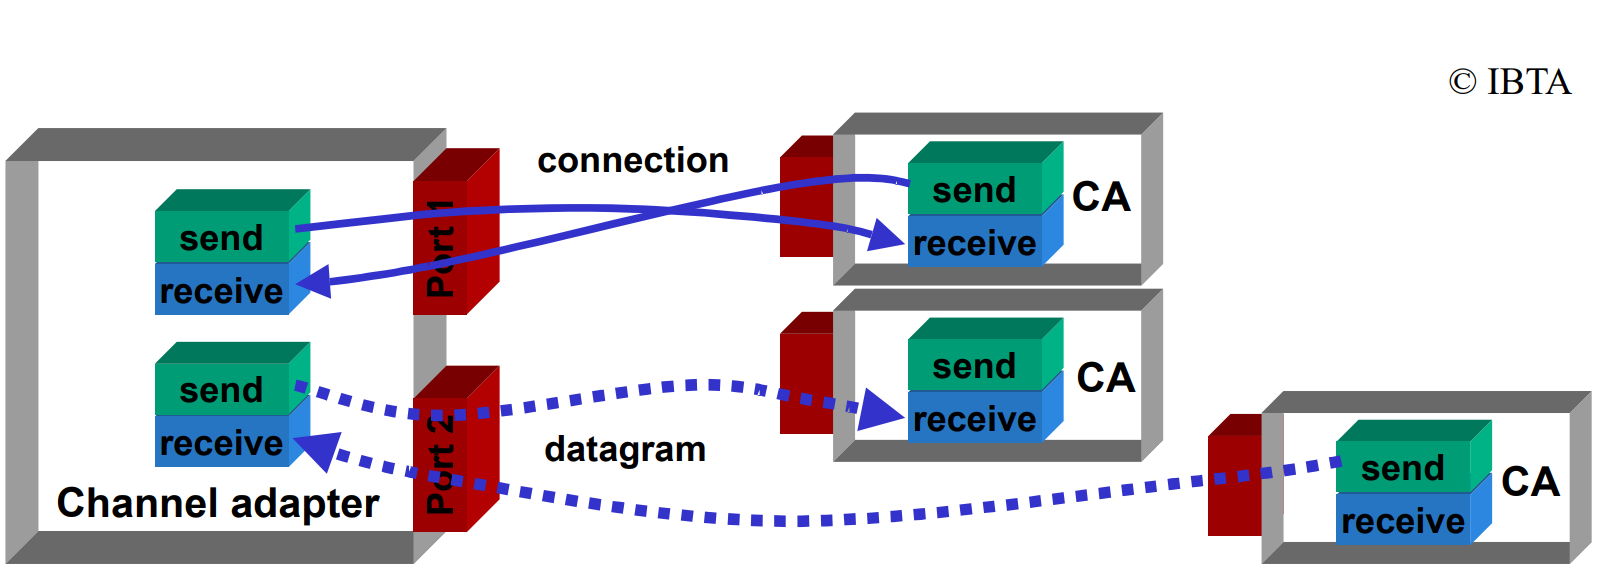
\includegraphics[width=0.6\textwidth]{image/chap01/qp.png}
	\caption{队列对(QP)示意图}
	\label{fig:qp}
\end{figure}

\begin{enumerate}
	\item 两端程序各自创建一个队列对,并借助套接字等基础通信方式,交换队列对的基本信息,建立一对连接。
	\item Infiniband通信的基本单位是一个(发送/接收/完成)事务:接收方通过Verbs调用将一个构造好的接收事务压入到接收队列(Receive Queue)中
	\item 之后发送方将一个构造好的发送事务压入到发送队列(Send Queue)中。
	\item 此时,硬件将为两端处理这一对事务,将本机内存从发送事务指定的内存地址发送到接收事务指定的远端内存地址。
	\item 硬件完成一次事务操作后,通常将一个完成队列项(CQE)压入到完成队列(Completion Queue,CQ)中。
	\item 用户进程可以在任何时刻通过弹出完成队列的头部来确认(发送/接收)事务执行完成,或者得到操作失败的错误代码。
\end{enumerate}

以上流程实现了类似TCP/UDP的双边通信语义,不过,两者仍然有着本质的区别:RDMA通信机制是基于事务模型的;以上操作均在用户态完成,无需任何系统调用;数据从一个进程直接发送到另一个进程。
除此之外,RDMA机制还支持使用读/写(Read/Write)等单边通信语义。在执行这些单边操作时,远端应用不需要事先发送接收事务,也不会通过完成队列得知通信的发生。
使用单边操作语义将会进一步降低远端CPU的介入和负担,从而支持更高强度的并发操作。不过,使用单边语义通常需要引入额外的同步机制以完成通信。

\subsection{基于RDMA技术的内存系统}

近年来,针对RDMA机制提供的高带宽、低延迟优势,研究人员在多个方向上尝试将其转变为实际应用上的性能提升。特别是在RDMA同时支持双边和单边语义的情况下,
如何针对实际应用场景,设计合适的通信和协作机制,一直是这一领域研究的重点。从场景的角度来说,目前的主要研究方向是分布式内存系统和高并发的内存系统。

\subsubsection{分布式内存系统}

Infiniband网络标准和RDMA技术最早应用于高性能计算(HPC)领域。俄亥俄州立大学的\cite{}首次将RDMA技术应用于优化消息传递接口(MPI)的通信机制,这也是最早的、较为完善的一个RDMA
协作机制实现。这一设计针对RDMA单边操作所产生的协作困难问题,预先建立了固定映射的发送-接收缓冲区对,以及设计了自描述的消息块,深刻影响了后续RDMA通信方案的设计。并且在MPI
多年的演进中,其RDMA通信机制也不断有优化方案提出。

然而,从集群内存空间的角度来看,RDMA技术的逐渐成熟,让研究者看到了颠覆性、普适性优化的可能性:优异的访问带宽和极低的访问延迟,已经极大程度地拉近了机器内存之间的“距离”,使得
集群规模的共享内存逐渐成为可能:\cite{}发现IB网络的通信延迟和PCIe总线上的通信延迟处于一个数量级,这说明网络已经不再是集群通信的性能瓶颈。以RDMA为核心,HPC社区和分布式系统社区均
提出了一些分布式共享内存的实现方案,从而以较低的性能代价连接起整个集群的内存空间:前者包括GasNet,OpenSHMEM等支持分区全局地址空间(PGAS)计算的中间件;后者以FaRM,CoRM等系统为代表。
这些研究的共同焦点是分布式的事务机制——除了本地内存的读-写冲突之外,还需要解决远端机器读写和本地访存之间的数据冲突。此外,也有研究避开了细粒度的内存管理,如去中心化、可扩展的
分布式页表系统Infiniswap,就通过粗粒度的内存页交换处理集群中存在的物理内存使用不均的问题。

\subsubsection{高并发内存系统}

在另一个方向上,研究人员希望将RDMA低延迟、高并发的特性直接变为应用的性能——内存键值对(key-value)数据库是一个合适的领域。Redis,Memcached等内存数据库通常被用作一种高速缓存,
其他机器对数据库的访问也主要以并发读取为主,因此非常适合使用RDMA技术进行优化,特别是使用单边读等通信方式优化单机并发能力。不过,基于单边操作的读取机制难以应对高强度并发中的数据冲突问题,
需要借助于更好的哈希函数等其他优化手段才能获得较好的优化效果。因此近期的工作更是提出了双边语义和单边语义混合的通信机制,从而在CPU负载、并发能力和编程难度上都获得较好的结果。
总体来说,在过去的一段时间,针对应用场景不同,研究人员已经提出了众多不同的RDMA通信范式。

\section{论文主要研究内容}

作为分布式计算框架Ray的核心组件,Plasma并没有对RDMA通信的支持,因而在超算集群中存在性能提升的空间。该组件兼有分布式、高并发两方面的特性:
作为集群内存存储,Plasma需要运行在集群的每个计算节点上,并且期望实现最大的并发传输能力,以支撑Ray快速的任务调度。
不过,Plasma并没有实现细粒度的并发机制,而是进一步依靠Redis等外部机制实现。这使得我们的研究重点倾向于优化大型数据对象的传输性能。
在本文中,我们为Plasma提出了一种原生支持RDMA技术的通信机制,并且在现代超算集群上验证了其在各个数据大小的传输上都获得了更优的性能。

这一工作存在以下挑战:

\begin{enumerate}
	\item 目前RDMA编程仍然是极为“小众”的技术,如何能在有限的资料和现有研究帮助下实现高性能的网络通信机制。
	\item 如何在尽可能不破坏项目整体结构的情况下,为Plasma提供原生RDMA通信机制。这要求优化后的程序可以无缝地运行在以太网和Infiniband两种网络架构上。
	\item 针对Ray框架中可能出现的大小不一的数据,如何实现该机制使得Plasma能够在尽可能多的大小范围内都能获得最优的网络性能。
\end{enumerate}

下面总结了本工作的主要贡献:

\begin{enumerate}
	\item 我们通过实验分析了原Plasma实现在超算集群上的存储和网络性能,验证了其无法充分利用Infiniband高速网络,从而证明了使用RDMA技术优化Plasma数据传输的可行性。
	\item 我们针对小对象数据和分布式训练中常见的大对象数据,分别实现了基于双边和单边通信的传输机制。针对大对象,单边通信将实现用户态的零拷贝特性,从而降低了CPU数据拷贝而导致的负载和占用时间。
	\item 我们基于消息传递接口MPI实现了分布式、可扩展的数据传输性能测试,比较了优化实现和原实现在各个数据大小上的性能。并且通过实验,我们确定了机制在选择传输方式时的最佳方案,从而获得了最优的整体性能。
\end{enumerate}

\section{论文结构与章节安排}
\label{sec:arrangement}

本文共分为五章,这些章节的内容安排如下:

第一章:绪论。简述了本文的研究背景和意义,简述了本研究的核心技术背景,并介绍了国内外相关工作和研究现状。

第二章:Plasma分布式内存存储的架构和性能分析。这一章将简要分析Plasma的分布式架构,并且通过性能测试和常见内存存储Redis进行对比,
分析了Plasma在传统网络结构上的性能瓶颈。

第三章:基于RDMA技术的混合通信机制实现。这一章将详细介绍基于RDMA技术的优化方案,并针对大小数据提出混合通信机制的实现。

第四章:实验和分析。这一章将在天河高性能集群上验证优化方案的性能优化,

第五章:总结和展望。这一章将总结本文的主要结果,并且进一步分析后续的工作方向。
